\begin{minipage}{0.265\textwidth}
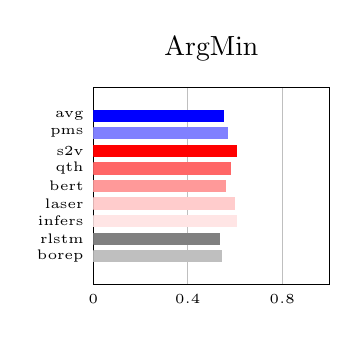
\begin{tikzpicture}

  	\begin{axis}[
		title=ArgMin,
 	   	xbar stacked,
		bar width=4pt,
		enlarge y limits=0.2,
    		symbolic y coords={borep,rlstm,infers,laser,bert,qth,s2v,pms,avg},
		xmin=0,xmax=1,
  		xmajorgrids,
		tickwidth=0pt,
		xtick distance=0.40,
  		ytick=data,
		scale only axis=true,
  		width=3cm,height=2.5cm,
		tick label style={font=\tiny}
  	]

		% avg
  		\addplot[blue,fill] coordinates
  			{(0.550,avg) (0.00,pms) (0.00,s2v) (0.00,qth) (0.00,bert) (0.00,laser) (0.00,infers) (0.00,rlstm) (0.00,borep)};
		% pms
		\addplot[blue!50,fill] coordinates
			{(0.00,avg) (0.568,pms) (0.00,s2v) (0.00,qth) (0.00,bert) (0.00,laser) (0.00,infers) (0.00,rlstm) (0.00,borep)};

		% s2v
		\addplot[red,fill] coordinates 
			{(0.00,avg) (0.00,pms) (0.608,s2v) (0.00,qth) (0.00,bert) (0.00,laser) (0.00,infers) (0.00,rlstm) (0.00,borep)};
		% qth
		\addplot[red!60,fill] coordinates
			{(0.00,avg) (0.00,pms) (0.00,s2v) (0.581,qth) (0.00,bert) (0.00,laser) (0.00,infers) (0.00,rlstm) (0.00,borep)};
		% bert
		\addplot[red!40,fill] coordinates
			{(0.00,avg) (0.00,pms) (0.00,s2v) (0.00,qth) (0.558,bert) (0.00,laser) (0.00,infers) (0.00,rlstm) (0.00,borep)};
		% laser
		\addplot[red!20,fill] coordinates
			{(0.00,avg) (0.00,pms) (0.00,s2v) (0.00,qth) (0.00,bert) (0.596,laser) (0.00,infers) (0.00,rlstm) (0.00,borep)};
		% infers
		\addplot[red!10,fill] coordinates
			{(0.00,avg) (0.00,pms) (0.00,s2v) (0.00,qth) (0.00,bert) (0.00,laser) (0.604,infers) (0.00,rlstm) (0.00,borep)};

		% rand lstm
		\addplot[gray,fill] coordinates 
			{(0.00,avg) (0.00,pms) (0.00,s2v) (0.00,qth) (0.00,bert) (0.00,laser) (0.00,infers) (0.536,rlstm) (0.00,borep)};
		% borep
		\addplot[lightgray,fill] coordinates 
			{(0.00,avg) (0.00,pms) (0.00,s2v) (0.00,qth) (0.00,bert) (0.00,laser) (0.00,infers) (0.00,rlstm) (0.542,borep)};

  	\end{axis}



\end{tikzpicture}
\end{minipage}
\hfill
\begin{minipage}{0.25\textwidth}
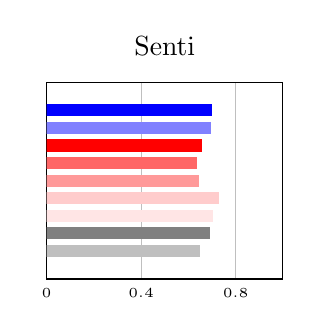
\begin{tikzpicture}

  	\begin{axis}[
		title=Senti,
   	 	xbar stacked,
		bar width=4pt,
		enlarge y limits=0.2,
	    	symbolic y coords={borep,rlstm,infers,laser,bert,qth,s2v,pms,avg},
		xmin=0,xmax=1,
  		xmajorgrids,
		tickwidth=0pt,
		xtick distance=0.40,
  		ytick=data,
		yticklabels={,,},
		scale only axis=true,
  		width=3cm,height=2.5cm,
		tick label style={font=\tiny}
  	]

		% avg
  		\addplot[blue,fill] coordinates
  			{(0.698,avg) (0.00,pms) (0.00,s2v) (0.00,qth) (0.00,bert) (0.00,laser) (0.00,infers) (0.00,rlstm) (0.00,borep)};
		% pms
		\addplot[blue!50,fill] coordinates
			{(0.00,avg) (0.695,pms) (0.00,s2v) (0.00,qth) (0.00,bert) (0.00,laser) (0.00,infers) (0.00,rlstm) (0.00,borep)};

		% s2v
		\addplot[red,fill] coordinates 
			{(0.00,avg) (0.00,pms) (0.656,s2v) (0.00,qth) (0.00,bert) (0.00,laser) (0.00,infers) (0.00,rlstm) (0.00,borep)};
		% qth
		\addplot[red!60,fill] coordinates
			{(0.00,avg) (0.00,pms) (0.00,s2v) (0.636,qth) (0.00,bert) (0.00,laser) (0.00,infers) (0.00,rlstm) (0.00,borep)};
		% bert
		\addplot[red!40,fill] coordinates
			{(0.00,avg) (0.00,pms) (0.00,s2v) (0.00,qth) (0.644,bert) (0.00,laser) (0.00,infers) (0.00,rlstm) (0.00,borep)};
		% laser
		\addplot[red!20,fill] coordinates
			{(0.00,avg) (0.00,pms) (0.00,s2v) (0.00,qth) (0.00,bert) (0.727,laser) (0.00,infers) (0.00,rlstm) (0.00,borep)};
		% infers
		\addplot[red!10,fill] coordinates
			{(0.00,avg) (0.00,pms) (0.00,s2v) (0.00,qth) (0.00,bert) (0.00,laser) (0.702,infers) (0.00,rlstm) (0.00,borep)};

		% rand lstm
		\addplot[gray,fill] coordinates 
			{(0.00,avg) (0.00,pms) (0.00,s2v) (0.00,qth) (0.00,bert) (0.00,laser) (0.00,infers) (0.688,rlstm) (0.00,borep)};
		% borep
		\addplot[lightgray,fill] coordinates 
			{(0.00,avg) (0.00,pms) (0.00,s2v) (0.00,qth) (0.00,bert) (0.00,laser) (0.00,infers) (0.00,rlstm) (0.646,borep)};

  	\end{axis}

\end{tikzpicture}
\end{minipage}
\hfill
\begin{minipage}{0.25\textwidth}
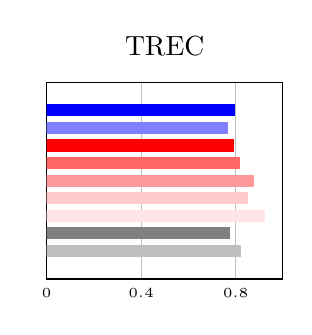
\begin{tikzpicture}

  	\begin{axis}[
		title=TREC,
 	   	xbar stacked,
		bar width=4pt,
		enlarge y limits=0.2,
    		symbolic y coords={borep,rlstm,infers,laser,bert,qth,s2v,pms,avg},
		xmin=0,xmax=1,
  		xmajorgrids,
		tickwidth=0pt,
		xtick distance=0.40,
  		ytick=data,
		yticklabels={,,},
		scale only axis=true,
  		width=3cm,height=2.5cm,
		tick label style={font=\tiny}
  	]

		% avg
  		\addplot[blue,fill] coordinates
  			{(0.795,avg) (0.00,pms) (0.00,s2v) (0.00,qth) (0.00,bert) (0.00,laser) (0.00,infers) (0.00,rlstm) (0.00,borep)};
		% pms
		\addplot[blue!50,fill] coordinates
			{(0.00,avg) (0.767,pms) (0.00,s2v) (0.00,qth) (0.00,bert) (0.00,laser) (0.00,infers) (0.00,rlstm) (0.00,borep)};

		% s2v
		\addplot[red,fill] coordinates 
			{(0.00,avg) (0.00,pms) (0.792,s2v) (0.00,qth) (0.00,bert) (0.00,laser) (0.00,infers) (0.00,rlstm) (0.00,borep)};
		% qth
		\addplot[red!60,fill] coordinates
			{(0.00,avg) (0.00,pms) (0.00,s2v) (0.814,qth) (0.00,bert) (0.00,laser) (0.00,infers) (0.00,rlstm) (0.00,borep)};
		% bert
		\addplot[red!40,fill] coordinates
			{(0.00,avg) (0.00,pms) (0.00,s2v) (0.00,qth) (0.876,bert) (0.00,laser) (0.00,infers) (0.00,rlstm) (0.00,borep)};
		% laser
		\addplot[red!20,fill] coordinates
			{(0.00,avg) (0.00,pms) (0.00,s2v) (0.00,qth) (0.00,bert) (0.851,laser) (0.00,infers) (0.00,rlstm) (0.00,borep)};
		% infers
		\addplot[red!10,fill] coordinates
			{(0.00,avg) (0.00,pms) (0.00,s2v) (0.00,qth) (0.00,bert) (0.00,laser) (0.920,infers) (0.00,rlstm) (0.00,borep)};

		% rand lstm
		\addplot[gray,fill] coordinates 
			{(0.00,avg) (0.00,pms) (0.00,s2v) (0.00,qth) (0.00,bert) (0.00,laser) (0.00,infers) (0.774,rlstm) (0.00,borep)};
		% borep
		\addplot[lightgray,fill] coordinates 
			{(0.00,avg) (0.00,pms) (0.00,s2v) (0.00,qth) (0.00,bert) (0.00,laser) (0.00,infers) (0.00,rlstm) (0.819,borep)};

  	\end{axis}

\end{tikzpicture}
\end{minipage}
%\hfill
%\begin{minipage}{0.2\textwidth}
%\begin{tikzpicture}
%
%  	\begin{axis}[
%		title=SUBJ,
% 	   	xbar stacked,
%		bar width=4pt,
%		enlarge y limits=0.2,
%    		symbolic y coords={rlstm,infers,laser,bert,qth,s2v,pms,avg},
%		xmin=0,xmax=1,
%  		xmajorgrids,
%		tickwidth=0pt,
%		xtick distance=0.40,
%  		ytick=data,
%		yticklabels={,,},
%		scale only axis=true,
%  		width=3cm,height=2cm,
%		tick label style={font=\tiny}
%  	]
%
%		% avg
%  		\addplot[blue,fill] coordinates
%  			{(0.908,avg) (0.00,pms) (0.00,s2v) (0.00,qth) (0.00,bert) (0.00,laser) (0.00,infers) (0.00,rlstm)};
%		% pms
%		\addplot[blue!50,fill] coordinates
%			{(0.00,avg) (0.896,pms) (0.00,s2v) (0.00,qth) (0.00,bert) (0.00,laser) (0.00,infers) (0.00,rlstm)};
%
%		% s2v
%		\addplot[red,fill] coordinates 
%			{(0.00,avg) (0.00,pms) (0.920,s2v) (0.00,qth) (0.00,bert) (0.00,laser) (0.00,infers) (0.00,rlstm)};
%		% qth
%		\addplot[red!60,fill] coordinates
%			{(0.00,avg) (0.00,pms) (0.00,s2v) (0.816,qth) (0.00,bert) (0.00,laser) (0.00,infers) (0.00,rlstm)};
%		% bert
%		\addplot[red!40,fill] coordinates
%			{(0.00,avg) (0.00,pms) (0.00,s2v) (0.00,qth) (0.928,bert) (0.00,laser) (0.00,infers) (0.00,rlstm)};
%		% laser
%		\addplot[red!20,fill] coordinates
%			{(0.00,avg) (0.00,pms) (0.00,s2v) (0.00,qth) (0.00,bert) (0.914,laser) (0.00,infers) (0.00,rlstm)};
%		% infers
%		\addplot[red!20,fill] coordinates
%			{(0.00,avg) (0.00,pms) (0.00,s2v) (0.00,qth) (0.00,bert) (0.00,laser) (0.912,infers) (0.00,rlstm)};
%
%		% rand lstm
%		\addplot[gray,fill] coordinates 
%			{(0.00,avg) (0.00,pms) (0.00,s2v) (0.00,qth) (0.00,bert) (0.00,laser) (0.00,infers) (0.903,rlstm)};
%
%  	\end{axis}
%
%\end{tikzpicture}
%\end{minipage}
%\hfill
%\begin{minipage}{0.1\textwidth}
%\begin{tikzpicture}
%
%  	\begin{axis}[
%		title=Cluster,
%   	 	xbar stacked,
%		bar width=4pt,
%		enlarge y limits=0.2,
%	    	symbolic y coords={rlstm,infers,laser,bert,qth,s2v,pms,avg},
%		xmin=0,xmax=1,
%  		xmajorgrids,
%		tickwidth=0pt,
%		xtick distance=0.40,
%  		ytick=data,
%		yticklabels={,,},
%		scale only axis=true,
%  		width=1.3cm,height=2cm,
%		tick label style={font=\tiny}
%  	]
%
%		% avg
%  		\addplot[blue,fill] coordinates
%  			{(0.00,avg) (0.00,pms) (0.00,s2v) (0.00,qth) (0.00,bert) (0.00,laser) (0.00,infers) (0.00,rlstm)};
%		% pms
%		\addplot[blue!50,fill] coordinates
%			{(0.00,avg) (0.00,pms) (0.00,s2v) (0.00,qth) (0.00,bert) (0.00,laser) (0.00,infers) (0.00,rlstm)};
%
%		% s2v
%		\addplot[red,fill] coordinates 
%			{(0.00,avg) (0.00,pms) (0.00,s2v) (0.00,qth) (0.00,bert) (0.00,laser) (0.00,infers) (0.00,rlstm)};
%		% qth
%		\addplot[red!60,fill] coordinates
%			{(0.00,avg) (0.00,pms) (0.00,s2v) (0.00,qth) (0.00,bert) (0.00,laser) (0.00,infers) (0.00,rlstm)};
%		% bert
%		\addplot[red!40,fill] coordinates
%			{(0.00,avg) (0.00,pms) (0.00,s2v) (0.00,qth) (0.00,bert) (0.00,laser) (0.00,infers) (0.00,rlstm)};
%		% laser
%		\addplot[red!20,fill] coordinates
%			{(0.00,avg) (0.00,pms) (0.00,s2v) (0.00,qth) (0.00,bert) (0.00,laser) (0.00,infers) (0.00,rlstm)};
%		% infers
%		\addplot[red!20,fill] coordinates
%			{(0.00,avg) (0.00,pms) (0.00,s2v) (0.00,qth) (0.00,bert) (0.00,laser) (0.00,infers) (0.00,rlstm)};
%
%		% rand lstm
%		\addplot[gray,fill] coordinates 
%			{(0.00,avg) (0.00,pms) (0.00,s2v) (0.00,qth) (0.00,bert) (0.00,laser) (0.00,infers) (0.00,rlstm)};
%
%  	\end{axis}
%
%\end{tikzpicture}
%\end{minipage}
%\hfill
%\begin{minipage}{0.1\textwidth}
%\begin{tikzpicture}
%
%  	\begin{axis}[
%		title=MR,
%    		xbar stacked,
%		bar width=4pt,
%		enlarge y limits=0.2,
%    		symbolic y coords={rlstm,infers,laser,bert,qth,s2v,pms,avg},
%		xmin=0,xmax=1,
%  		xmajorgrids,
%		tickwidth=0pt,
%		xtick distance=0.40,
%  		ytick=data,
%		yticklabels={,,},
%		scale only axis=true,
%  		width=1.3cm,height=2cm,
%		tick label style={font=\tiny}
%  	]
%
%		% avg
%  		\addplot[blue,fill] coordinates
%  			{(0.763,avg) (0.00,pms) (0.00,s2v) (0.00,qth) (0.00,bert) (0.00,laser) (0.00,infers) (0.00,rlstm)};
%		% pms
%		\addplot[blue!50,fill] coordinates
%			{(0.00,avg) (0.753,pms) (0.00,s2v) (0.00,qth) (0.00,bert) (0.00,laser) (0.00,infers) (0.00,rlstm)};
%
%		% s2v
%		\addplot[red,fill] coordinates 
%			{(0.00,avg) (0.00,pms) (0.763,s2v) (0.00,qth) (0.00,bert) (0.00,laser) (0.00,infers) (0.00,rlstm)};
%		% qth
%		\addplot[red!60,fill] coordinates
%			{(0.00,avg) (0.00,pms) (0.00,s2v) (0.633,qth) (0.00,bert) (0.00,laser) (0.00,infers) (0.00,rlstm)};
%		% bert
%		\addplot[red!40,fill] coordinates
%			{(0.00,avg) (0.00,pms) (0.00,s2v) (0.00,qth) (0.683,bert) (0.00,laser) (0.00,infers) (0.00,rlstm)};
%		% laser
%		\addplot[red!20,fill] coordinates
%			{(0.00,avg) (0.00,pms) (0.00,s2v) (0.00,qth) (0.00,bert) (0.751,laser) (0.00,infers) (0.00,rlstm)};
%		% infers
%		\addplot[red!20,fill] coordinates
%			{(0.00,avg) (0.00,pms) (0.00,s2v) (0.00,qth) (0.00,bert) (0.00,laser) (0.748,infers) (0.00,rlstm)};
%
%		% rand lstm
%		\addplot[gray,fill] coordinates 
%			{(0.00,avg) (0.00,pms) (0.00,s2v) (0.00,qth) (0.00,bert) (0.00,laser) (0.00,infers) (0.745,rlstm)};
%
%  	\end{axis}
%
%\end{tikzpicture}
%\end{minipage}
%\hfill
%\begin{minipage}{0.1\textwidth}
%\begin{tikzpicture}
%
%  	\begin{axis}[
%		title=MPQA,
%  	  	xbar stacked,
%		bar width=4pt,
%		enlarge y limits=0.2,
%    		symbolic y coords={rlstm,infers,laser,bert,qth,s2v,pms,avg},
%		xmin=0,xmax=1,
%  		xmajorgrids,
%		tickwidth=0pt,
%		xtick distance=0.40,
%  		ytick=data,
%		yticklabels={,,},
%		scale only axis=true,
%  		width=1.3cm,height=2cm,
%		tick label style={font=\tiny}
%  	]
%
%		% avg
%  		\addplot[blue,fill] coordinates
%  			{(0.848,avg) (0.00,pms) (0.00,s2v) (0.00,qth) (0.00,bert) (0.00,laser) (0.00,infers) (0.00,rlstm)};
%		% pms
%		\addplot[blue!50,fill] coordinates
%			{(0.00,avg) (0.841,pms) (0.00,s2v) (0.00,qth) (0.00,bert) (0.00,laser) (0.00,infers) (0.00,rlstm)};
%
%		% s2v
%		\addplot[red,fill] coordinates 
%			{(0.00,avg) (0.00,pms) (0.848,s2v) (0.00,qth) (0.00,bert) (0.00,laser) (0.00,infers) (0.00,rlstm)};
%		% qth
%		\addplot[red!60,fill] coordinates
%			{(0.00,avg) (0.00,pms) (0.00,s2v) (0.724,qth) (0.00,bert) (0.00,laser) (0.00,infers) (0.00,rlstm)};
%		% bert
%		\addplot[red!40,fill] coordinates
%			{(0.00,avg) (0.00,pms) (0.00,s2v) (0.00,qth) (0.809,bert) (0.00,laser) (0.00,infers) (0.00,rlstm)};
%		% laser
%		\addplot[red!20,fill] coordinates
%			{(0.00,avg) (0.00,pms) (0.00,s2v) (0.00,qth) (0.00,bert) (0.855,laser) (0.00,infers) (0.00,rlstm)};
%		% infers
%		\addplot[red!20,fill] coordinates
%			{(0.00,avg) (0.00,pms) (0.00,s2v) (0.00,qth) (0.00,bert) (0.00,laser) (0.836,infers) (0.00,rlstm)};
%
%		% rand lstm
%		\addplot[gray,fill] coordinates 
%			{(0.00,avg) (0.00,pms) (0.00,s2v) (0.00,qth) (0.00,bert) (0.00,laser) (0.00,infers) (0.851,rlstm)};
%
%  	\end{axis}
%
%\end{tikzpicture}
%\end{minipage}
%\hfill
%\begin{minipage}{0.1\textwidth}
%\begin{tikzpicture}
%
%  	\begin{axis}[
%		title=CR,
% 	   	xbar stacked,
%		bar width=4pt,
%		enlarge y limits=0.2,
%    		symbolic y coords={rlstm,infers,laser,bert,qth,s2v,pms,avg},
%		xmin=0,xmax=1,
%  		xmajorgrids,
%		tickwidth=0pt,
%		xtick distance=0.40,
%  		ytick=data,
%		yticklabels={,,},
%		scale only axis=true,
%  		width=1.3cm,height=2cm,
%		tick label style={font=\tiny}
%  	]
%
%		% avg
%  		\addplot[blue,fill] coordinates
%  			{(0.772,avg) (0.00,pms) (0.00,s2v) (0.00,qth) (0.00,bert) (0.00,laser) (0.00,infers) (0.00,rlstm)};
%		% pms
%		\addplot[blue!50,fill] coordinates
%			{(0.00,avg) (0.743,pms) (0.00,s2v) (0.00,qth) (0.00,bert) (0.00,laser) (0.00,infers) (0.00,rlstm)};
%
%		% s2v
%		\addplot[red,fill] coordinates 
%			{(0.00,avg) (0.00,pms) (0.751,s2v) (0.00,qth) (0.00,bert) (0.00,laser) (0.00,infers) (0.00,rlstm)};
%		% qth
%		\addplot[red!60,fill] coordinates
%			{(0.00,avg) (0.00,pms) (0.00,s2v) (0.675,qth) (0.00,bert) (0.00,laser) (0.00,infers) (0.00,rlstm)};
%		% bert
%		\addplot[red!40,fill] coordinates
%			{(0.00,avg) (0.00,pms) (0.00,s2v) (0.00,qth) (0.744,bert) (0.00,laser) (0.00,infers) (0.00,rlstm)};
%		% laser
%		\addplot[red!20,fill] coordinates
%			{(0.00,avg) (0.00,pms) (0.00,s2v) (0.00,qth) (0.00,bert) (0.802,laser) (0.00,infers) (0.00,rlstm)};
%		% infers
%		\addplot[red!20,fill] coordinates
%			{(0.00,avg) (0.00,pms) (0.00,s2v) (0.00,qth) (0.00,bert) (0.00,laser) (0.711,infers) (0.00,rlstm)};
%
%		% rand lstm
%		\addplot[gray,fill] coordinates 
%			{(0.00,avg) (0.00,pms) (0.00,s2v) (0.00,qth) (0.00,bert) (0.00,laser) (0.00,infers) (0.761,rlstm)};
%
%  	\end{axis}
%
%\end{tikzpicture}
%\end{minipage}